\RaggedRight
\setlength{\parindent}{2em} %首行缩进
\newpage

\title{影像辨識} %標題
\author{Chen Xiang-Wei} %編輯這份講義的作者

\date{\today}%今天
\date{\ROCtoday}%中華民國年
\lfoot{Author:\theauthor}
\maketitle
\thispagestyle{fancy}
\raggedright
\rhead{影像辨識}
%\tableofcontents  % 生成目錄
%請在以下輸入內容



\section{概論}

\subsection{機器學習}

機器學習是一種尋找目標函數的方法,常見的任務包含 Regression, Classification。舉例而言,若要用前三天的氣溫預測明天的氣溫,即是要找到 f,滿足: 

$$
f(\mbox{前三天的氣溫}) = \mbox{明天的氣溫}
$$

接著如果假設 f 是前三天氣溫的線性函數我們可以寫成

$$
t_{tomorrow}=y= b + w_1t_1+w_2t_2+w_3t_3
$$

當然現在不知道 $w_i, b$ 是多少。我們稱現在這個猜測的形式為 model,要找的$w_i, b$ 稱為weight。機器學習就是要用現有的數據 (Training data)去找出 weight,在這個例子中我們要可能需要蒐集前100天的氣溫資料。

\subsubsection*{Loss function 與 gradient descent}
一開始會隨機的初始化 weight,而 Loss function 則用於評估目前找到的函數和真實數據的差距。剛剛的例子中對於某一筆數據,真實的氣溫為 $\hat{y}$,前三天的氣溫為$X$,則預測函數 

$$
y= b + W\cdot X
$$
 
可以取 Loss function

$$
L = \frac{1}{n}\sum_{n} |\hat{y}-y|
$$

當然 Loss function不是唯一的,可以根據情況選擇合適的 loss,例如在 Classification 任務中,常會用 Cross-Entropy Loss。 

現在我們的目標可以寫成:

$$
\mbox{find:}\ w^*, b^* = \min_{w,b} L
$$

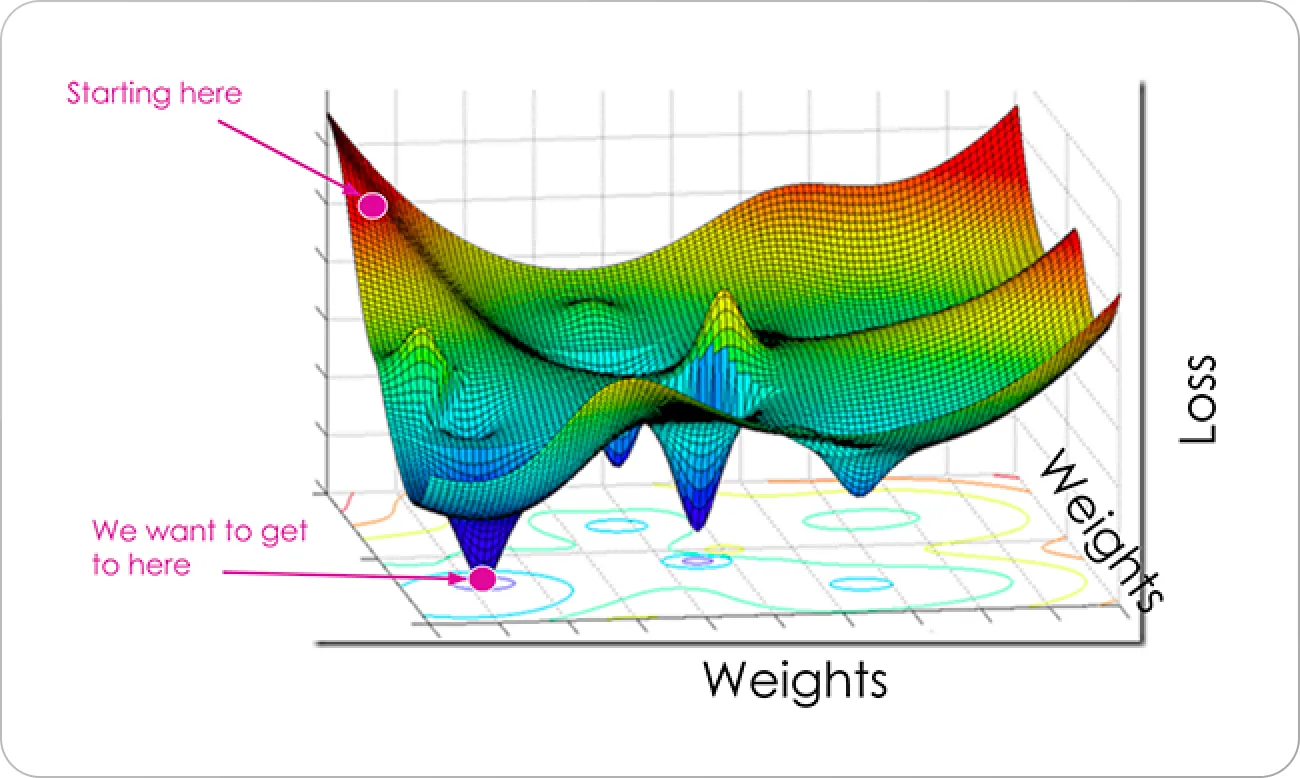
\includegraphics[width=.6\textwidth]{paste_src/2025-03-20-03-16-44.png}

\textbf{Gradient descent (梯度下降)}是找到 $w^*, b^*$的方法。如上圖,從 starting 開始,我們每次朝微分方向邁出一步,逐漸走到最低點,即:

$$w = w_0+\alpha\frac{\partial L}{\partial w}|_{w=w_0} \quad\alpha \mbox{: Learinig rate}$$

Learinig rate 是一步的步長。過短導致 loss 下降效率低,過長可能找不到最低點
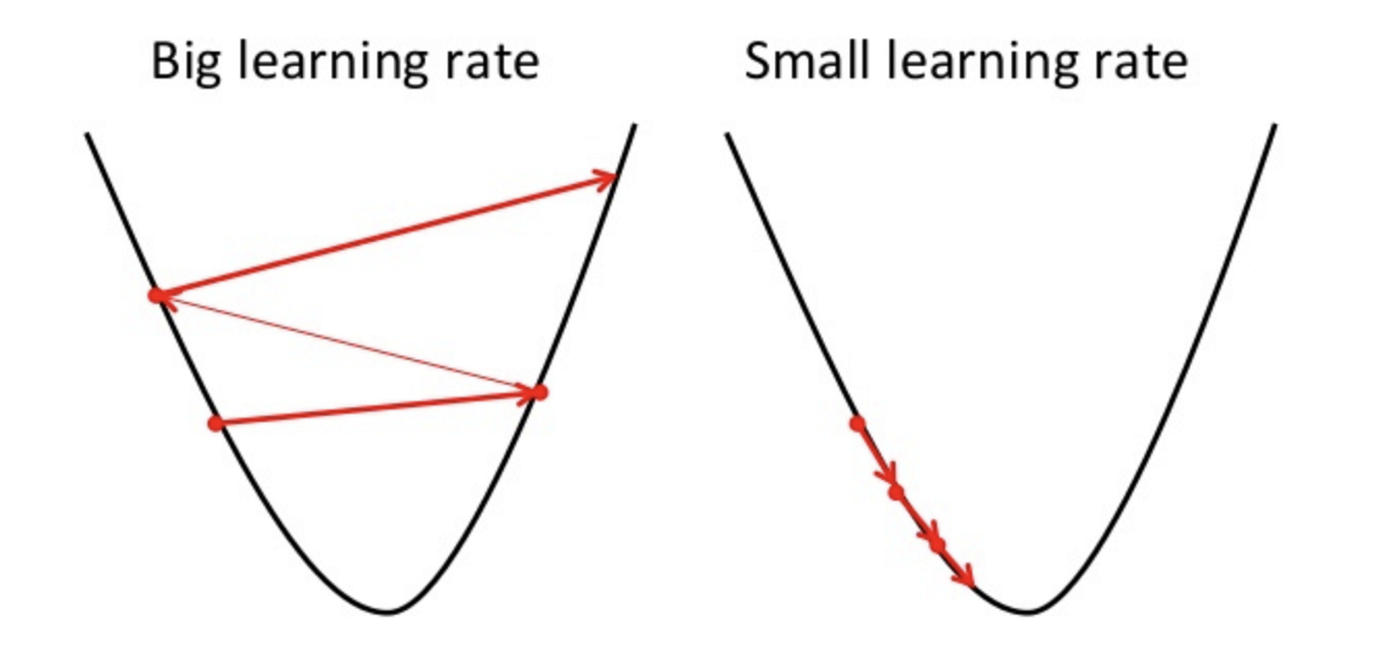
\includegraphics[width=.6\textwidth]{paste_src/2025-03-20-05-09-19.png}

\subsection{Optimizer}
Optimizer 即調整 Learinig rate 的方法,大部分用 adam 最穩定 (結合 momentum + RMSProp)

原本的 Gradient descent 可以寫成 

$$ 
w_{t+1}= w_t + \alpha g_t 
$$

$$
\mbox{Simple Idea: time dependent decay} \quad \alpha^t = \frac{\alpha}{\sqrt{t+1}}
$$






\subsubsection*{Adagrad} 

\begin{align}
  w_{t+1} &= w_t + \frac{\alpha_t}{\sigma_t} g_t \qquad \sigma_t: \mbox{root mean square of previous g}
\end{align}

越走越慢,root mean square 考慮了二次微分的影響


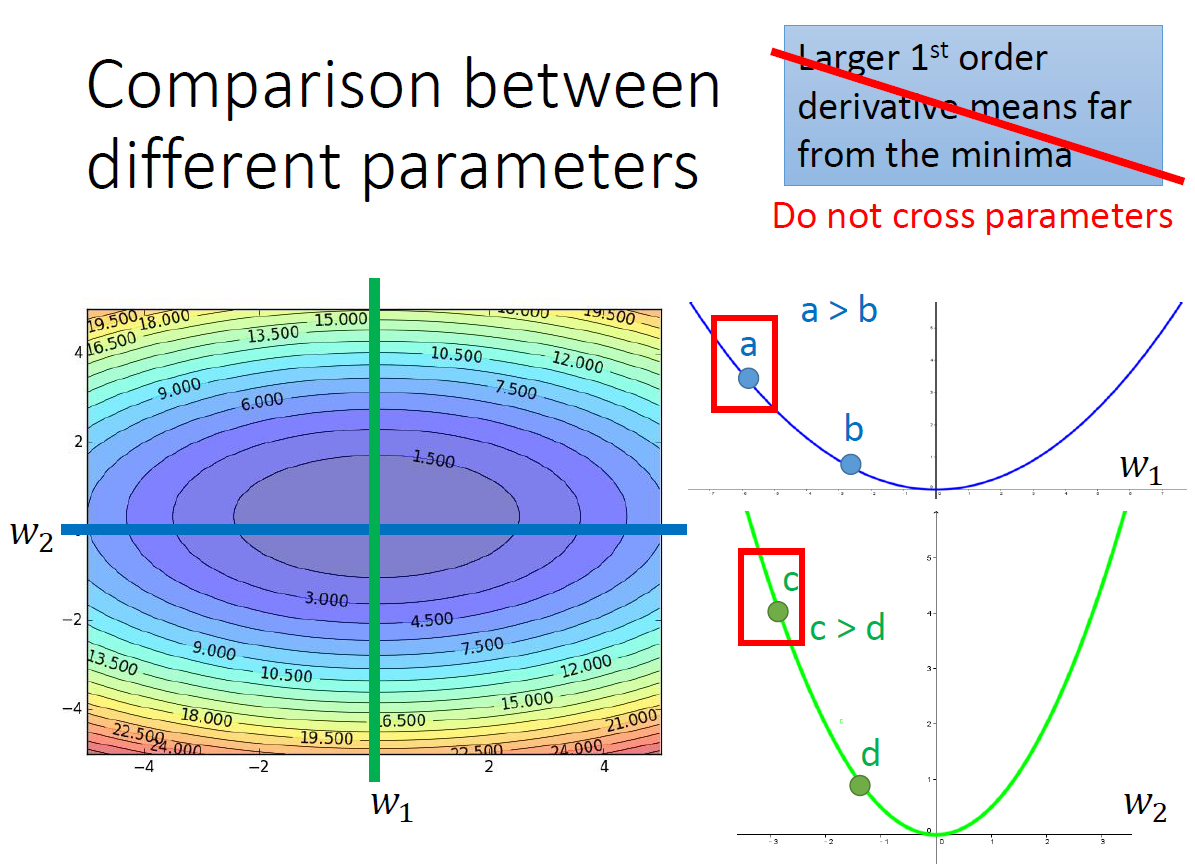
\includegraphics[width=.8\textwidth]{paste_src/2025-03-20-06-21-55.png}
\subsubsection*{Momentum}
如果上一次的梯度跟這次同方向的話,$|v|$會越來越大,$\mu$用以減少學習率震盪

\begin{align}
  v_{t+1} &= \mu v_{t} + (1-\mu) g_t \\
  w_{t+1} &= w_t + \alpha v_{t+1}
\end{align}





\subsection{Activation Function}
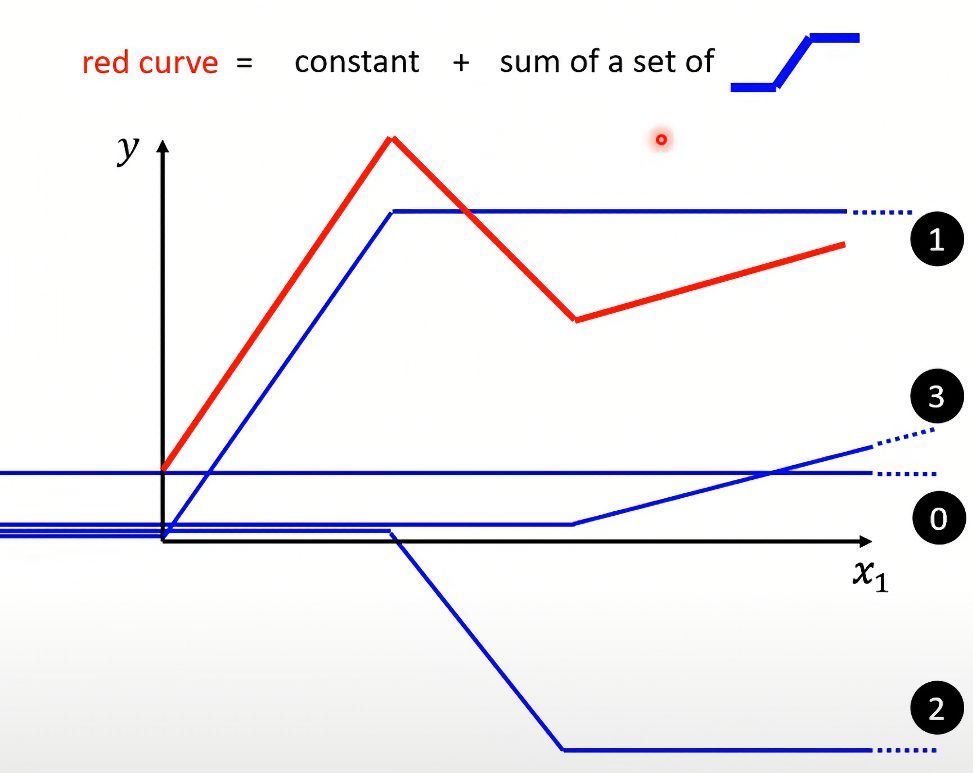
\includegraphics[width=.6\textwidth]{paste_src/2025-03-20-03-47-32.png}

線性函數的 model 解決不了大部分的問題,所以機器學習的 model 會引入 S 型的函數作為 Activation Function,例如 Sigmoid function:
$$
y= \frac{1}{1+e^x}
$$
所以最後的 model 會形如 
$$
\mbox{let}\quad r = b + Wx 
$$
$$
y = b'+\sum_i c_i \frac{1}{1+e^{r}} = b' + \sum_i c_i Sigmoid(r) = b' + C^TSigmoid(r)
$$
其中 C, b' 都是 weight。


如果我們把輸出的 y 當作 x 繼續重複疊 r 和 sigmoid 層就是神經網路 Neural Network 或 Deep learning,放在中間的層叫做 Hidden layer。

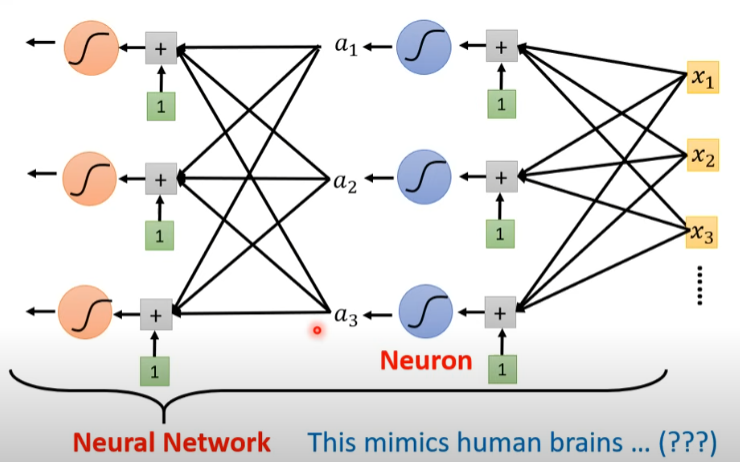
\includegraphics[width=.8\textwidth]{paste_src/2025-03-20-14-24-18.png}

\subsection*{Batch and epoch}

訓練資料會非常多,在實際做 gradient descent 的時候不會一次對所有資料算 loss,而是將資料隨機分成數個 Batch ,每次用一個 Batch 裡面的資料算 loss 和 gradient 來更新 weight。所有的 Batch 都用過一輪叫做一個 Epoch。

Batch 如果取的小,每個 Epoch 會更新 weight 很多次,計算效率較低。但每個 Batch 就較不能代表整體,所以算出來的 gradient 變化大,Loss 收斂較不穩定,但或許能跳出區間最小值。

每次在計算 gradient 的時候 Batch 的數據會被丟進 GPU 顯存。如果 Batch 太大顯存放不下,電腦會報記憶體錯誤,這時候只能減少 Batch。

\subsection{Classification} 

要讓函數輸出類別,最直觀的方法是 One-Hot Encoding。如果有 $N$ 類,就構建 N 維向量代表每個類別,形如: 

\begin{align*}
  &[ 1\ 0\ 0 \dots 0]\\
  &[ 0\ 1\ 0 \dots 0]\\
  &\vdots \\
  &[ 0\ 0\ 0 \dots 1]
\end{align*}
這樣就能讓模型輸出類別。


但這麼做在 N 很大的時候會大幅增加資料的維度,讓模型參數量暴增。另外, One-Hot Encoding 也假設了這些類別間彼此獨立。如果要做的分類任務的類別彼此相關,又數量很多,例如詞彙預測,One-Hot Encoding 就不是好方法。






\section{ 除錯 }

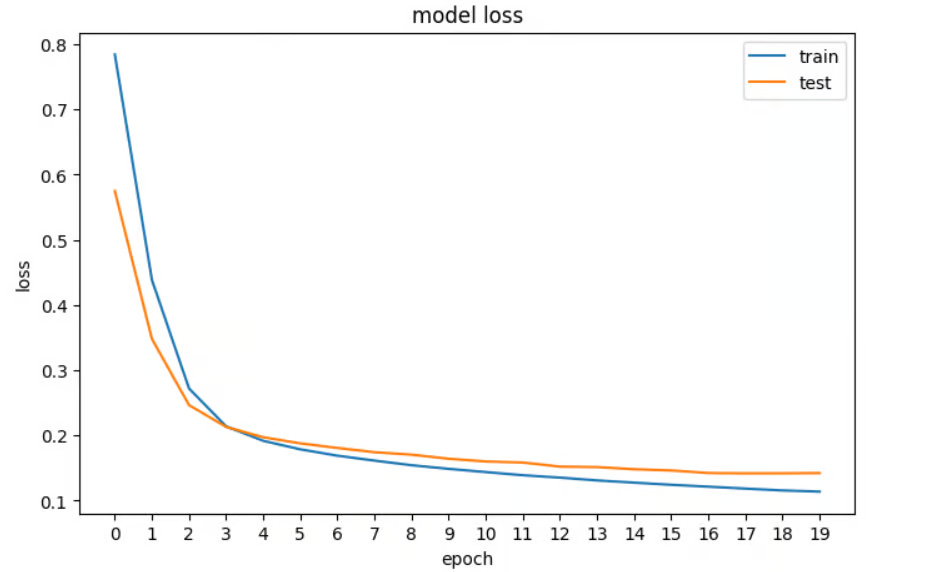
\includegraphics[width=.8\textwidth]{paste_src/2025-03-20-04-20-03.png}

預測結果很爛?先看 Training data 的 loss 除錯。一個好的 loss 應該要像上圖,除錯流程如下:



\begin{forest}
  [loss on train data 
    [large
      [model bias]
      [optimization]
    ]
    [small
      [loss on testing data
        [large
          [overfitting]
          [mismatch]
        ]
      ]
    ]
  ]
\end{forest}

\subsection*{Model Bias}
要找的function 不在 model 裡面
\begin{itemize}
  \item 使用更複雜或更有彈性的模型。
  \item 增加 Training data,提高數據多樣性。
  \item 增加更多有意義的特徵。
\end{itemize}

\subsection*{Optimization}

梯度下降法不能讓 Loss 無法有效降低
\begin{itemize}
  \item Learning rate (過大、過小或不合適的優化器)
  \item 梯度消失或梯度爆炸
\end{itemize}

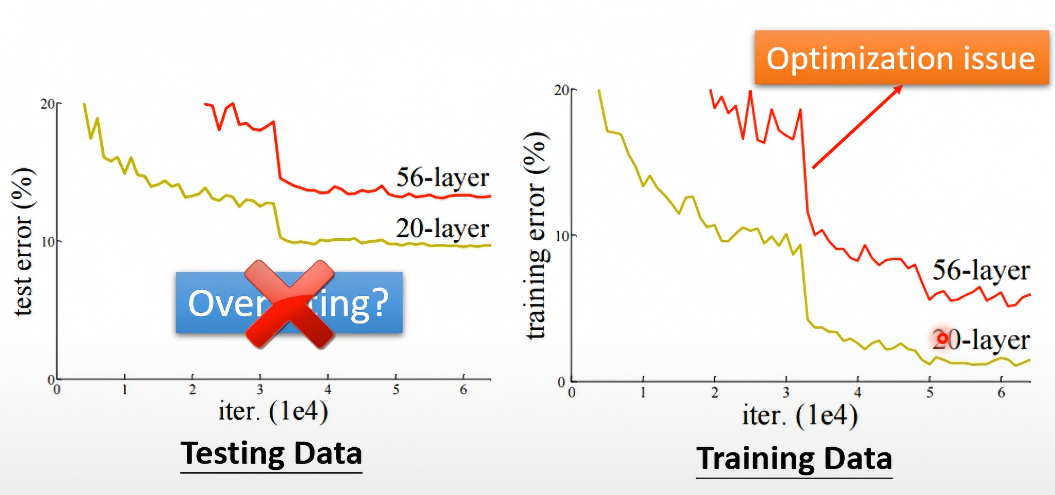
\includegraphics[width=1\textwidth]{paste_src/2025-03-20-04-48-18.png}



\subsection*{Overfitting}

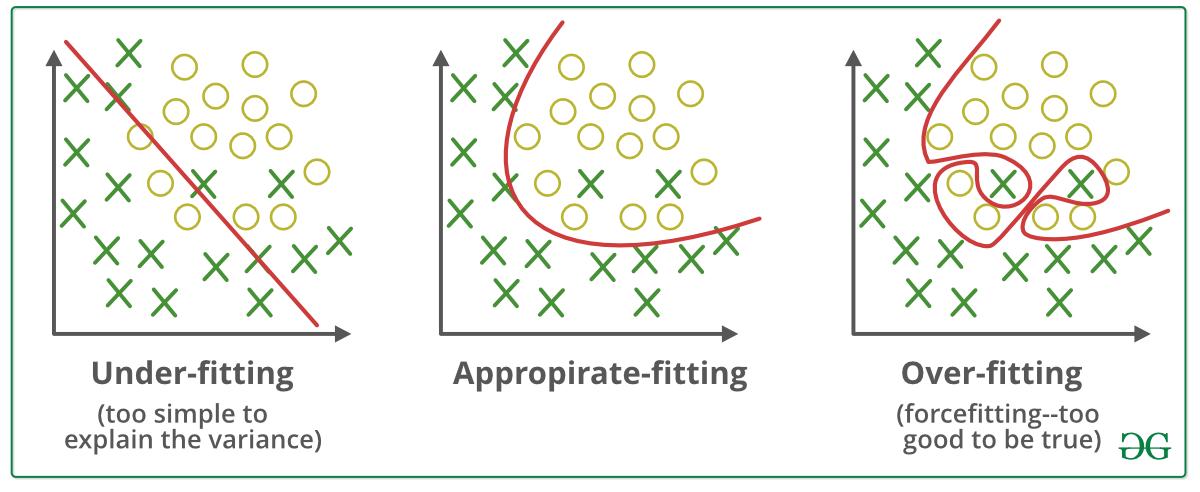
\includegraphics[width=1\textwidth]{paste_src/2025-03-20-04-57-13.png}

\begin{itemize}
  \item 增加訓練資料
  \item 減少 model 彈性 
\end{itemize}
